\documentclass[11pt,a4paper]{article}
\usepackage[T1]{fontenc}\usepackage[utf8]{inputenc}\usepackage[scaled=0.95]{helvet}\renewcommand{\familydefault}{\sfdefault}
\usepackage[a4paper,margin=2.2cm]{geometry}\usepackage{graphicx,booktabs,longtable,amsmath,caption}\usepackage[hidelinks]{hyperref}
\captionsetup{font=small,labelfont=bf}\setlength{\parindent}{0pt}\setlength{\parskip}{0.6em}
\begin{document}
{\LARGE\textbf{Parking around rue de Terrebonne: supply, measured demand, and the survey\textquoteright{}s answers in context}}\\[4pt]
{\small Terrebonne-open-sources, 2026-11-07. Author: a resident of Côte-des-Neiges--Notre-Dame-de-Grâce (see the repository\textquoteright{}s « About the author »). Companion to the note on winter bicycle counts and user frequency. Data: EXP 2023 (the borough\textquoteright{}s published study), City LiDAR 2015 and assessment roll (open data, CC-BY 4.0), Québec orthophoto, BAnQ plans, ECCC, City snow-removal transactions, the APC-NDG survey\textquoteright{}s anonymized file. Code, tables and figures: \url{https://github.com/OpenMobilityData/Terrebonne-open-sources/tree/main/2026-parking-supply-demand-survey-context}.}

\section*{Abstract}
The APC-NDG survey of October--November 2026 reports, for residents on rue de Terrebonne or within one block, how many keep a vehicle, how many have an off-street place, where the car was parked last night and how often winter parking was hard. Those are counts of respondents. This note places them against the measurements that exist of the parking they describe: the borough\textquoteright{}s 2023 study (EXP), which inventoried 478 on-street places on Terrebonne and 629 on the cross-street stubs within 50 m and measured their occupancy on a Thursday and a Saturday of September--October 2022; the 2015 City LiDAR night and a daytime orthophoto, on which the cars at Terrebonne\textquoteright{}s curbs were counted block by block before the 2024 lane; the 1954--55 insurance plans and present-day imagery, which give the share of buildings with a garage or driveway; the City assessment roll, which gives the dwellings; and five winters of snow-removal records. EXP found occupancy below its own 80\,\% threshold at every period in every sector: at 18:30--19:30 on the Thursday, 247 cars occupied 50\,\% of Terrebonne\textquoteright{}s places, leaving 246 vacant there and 298 on the stubs. The 2015 night count found 183 cars at the curbs, 37\,\% of the 2022 supply, rising from 28\,\% in the west sector to 46\,\% in the east. Both measurements of demand before the lane are of the order of the supply that remains on one side today (about 239 places). On Terrebonne itself, 72\,\% of buildings and 70\,\% of dwellings have a garage or driveway; the survey\textquoteright{}s respondents on the street report an off-street place in 18 of 35 households with a vehicle (51\,\%, interval 36--67\,\%), those within a block in 43 of 59. The survey\textquoteright{}s 60 street parkers and 35 reports of strict winter hardship are floors under a population of 573 dwellings on Terrebonne and 5,029 within a block, of which the survey reached 6\,\% and 1\,\%. The conditions the hardship questions describe occurred on about 32 nights a winter over the last five, 23 of them with snow loading. No measurement of present-day occupancy, with the lane in place, exists; the first parking analysis the borough has commissioned since 2022 is due on November 27, 2026.

\section*{Lay summary}
The survey asked people living on rue de Terrebonne or within a block about their parking. They count the people who replied, not the street. This note sets them beside the measurements on record: the borough\textquoteright{}s 2023 study (places and their occupancy on two days in 2022), a 2015 night laser survey, the 1954 insurance plans with today\textquoteright{}s aerial imagery, the City\textquoteright{}s roll of dwellings, and five winters of snow-loading records.

The 2023 study found half of Terrebonne\textquoteright{}s places empty on the Thursday evening; the 2015 night count found 183 cars along the street, one place in three. Both, taken before the lane, are close to today\textquoteright{}s supply on one side. Seven in ten homes on Terrebonne have a garage or driveway; respondents on the street reported one less often, within what 35 answers can show. The survey\textquoteright{}s 60 street parkers and 35 reports of winter difficulty are floors under 573 dwellings on the street and 5,029 nearby; snow loading constrained parking on about 32 nights a winter, 23 loading nights. Nobody has measured how full the street is now, lane in place.

\tableofcontents

\section{Question}
The companion note placed the survey\textquoteright{}s count of winter cyclists against the bicycle counters. This note does the same for its parking answers. The survey counts respondents: corridor residents who keep a vehicle, who have an off-street place, who parked on a street last night, who met the survey\textquoteright{}s definition of winter hardship. The measurements that exist of the same street are of a different kind: an inventory of places and their occupancy on two days (EXP, 2022), two snapshots of the cars at the curbs before the lane (LiDAR 2015; orthophoto), a reading of off-street parking building by building (the 1954--55 plans and present-day imagery), the dwellings on the roll, and the nights of snow-removal constraint. The questions are the same as before: what do the external measurements say about the population the respondents come from; can the survey\textquoteright{}s shares be checked against a ground truth; and what do the counts leave unmeasured.

\section{Data}
\begin{itemize}
\item \textbf{EXP 2023} (Étude de mobilité sur la rue de Terrebonne, September 2023, the borough\textquoteright{}s published study). Supply (report p.~40): 230 on-street places in the westbound direction and 248 eastbound on Terrebonne; 328 north and 301 south on the first 50~m of the cross streets. Occupancy and vacant places by sector (west, St-Ignatius--Cavendish; institutional, Cavendish--Grand; east, Grand--Girouard), by direction or side and by period, on Thursday, September 29, 2022 (7:30--8:30, 12:30--13:30, 18:30--19:30) and Saturday, October 1 (8:00--9:00, 12:30--13:30, 18:30--19:30): Tables 3-2 (p.~43) and 3-3 (p.~48), transcribed in \texttt{exp2023\_parking\_tables\_transcribed.csv}. Works between Walkley and Cumberland at the time (p.~4). Table 7-1 (p.~88): 475 places in the existing situation, 375 after bringing the street to standards, 161--172 under the three concepts.
\item \textbf{Cars at the curbs before the lane}: per block, both curbs, from the City\textquoteright{}s 2015 airborne LiDAR (a weeknight; cars read by eye on the height raster, 183) and from the Québec orthophoto (daytime, undated, before the 2024 lane; 158), as read for the 1954-plans work (\texttt{1954-underwriters-plans-terrebonne-garages}). Two snapshots, not a before-and-after.
\item \textbf{Off-street parking}: the 1954--55 Underwriters\textquoteright{} plans (garage as built) and present-day imagery (driveway or apron) for the 123 residential buildings with a Terrebonne address on the sixteen sheets available, joined to the roll for dwellings (268).
\item \textbf{Dwellings}: the City assessment roll (open data), units with a centroid between avenue Somerled (260~m north of the lane\textquoteright{}s axis) and avenue de Monkland (286~m south), along the lane from its west end to Girouard, the two avenues\textquoteright{} own frontages included; the survey\textquoteright{}s « within one block » band.
\item \textbf{Survey}: the anonymized file as of 2026-11-07 (206 responses; the public filing of November 2 reports 205), with the criteria of the filing\textquoteright{}s methods page: a street parker ticked Terrebonne, a cross street or Somerled/Monkland for last night; strict hardship = ten minutes or more to find a space or a space two blocks or more away on a typical evening, or, after a storm or during loading, a car two blocks or more away, a ticket, a tow or a car moved out of the neighbourhood; loose adds « took much longer to find a space ».
\item \textbf{Winters}: nights with snow removal pending or under way and nights with loading, December~1 to March~31, 2021--22 to 2025--26, for the borough and for Terrebonne\textquoteright{}s sector CDN-301 (City snow-removal transactions and ECCC; computed in the author\textquoteright{}s decision model).
\end{itemize}

\section{Method}
EXP gives, for each sector and side, the occupancy rate and the number of vacant places at each period; the supply of that sector and side is recovered as vacant $/(1 - \text{rate})$ and taken as the median over the six periods (sum 496 on Terrebonne and 610 on the stubs against the stated 478 and 629; the difference is rounding in the published rates). Occupied places per period follow. The curb counts are summed by block and by sector and set against the EXP supply of the same sector. The survey\textquoteright{}s shares carry 95\,\% Wilson intervals; the comparison with the plans-and-imagery reading is made on respondents on Terrebonne itself (the reading covers Terrebonne addresses only) and on those within a block. Coverage is respondents divided by dwellings on the roll, a share of dwellings rather than of households.

\section{Results}
\subsection{What EXP measured in 2022}
\begin{table}[htbp]\centering\small\caption{Occupied and vacant places by period, September 29 and October 1, 2022 (EXP Tables 3-2 and 3-3; supply derived as described).}\label{tab:per}
\begin{tabular}{@{}lrrrrrr@{}}\toprule period & Terrebonne occupied & vacant & occupancy & stubs occupied & vacant & occupancy\\ \midrule
Thu 7:30–8:30 & 276 & 221 & 56\,\% & 320 & 283 & 53\,\% \\
Thu 12:30–13:30 & 309 & 188 & 62\,\% & 346 & 267 & 56\,\% \\
Thu 18:30–19:30 & 247 & 246 & 50\,\% & 311 & 298 & 51\,\% \\
Sat 8:00–9:00 & 219 & 261 & 46\,\% & 306 & 304 & 50\,\% \\
Sat 12:30–13:30 & 216 & 279 & 44\,\% & 298 & 315 & 49\,\% \\
Sat 18:30–19:30 & 218 & 276 & 44\,\% & 264 & 343 & 44\,\% \\
\bottomrule\end{tabular}\end{table}
Occupancy on Terrebonne as a whole never exceeded 62\,\% at any period, and no sector-and-direction cell exceeded 71\,\% on Terrebonne or 76\,\% on the stubs (institutional, cross streets north, Thu AM). At the Thursday evening period, the closest the survey comes to a residential evening, 247 cars occupied 50\,\% of the places on Terrebonne, with 246 vacant on the street and 298 on the stubs; the east sector was the fullest (138 occupied, 84 vacant). EXP\textquoteright{}s own reading (p.~43 and p.~48) is that rates below 80\,\% leave flexibility, and its Table 7-1 projects the concepts\textquoteright{} 161--172 remaining places against 375 after standards, with the residual capacity by sector and period in Tables 7-2 to 7-4 (pp.~89--90), where it notes that occupancy may be locally higher near Girouard, Grand and Walkley.
\begin{figure}[htbp]\centering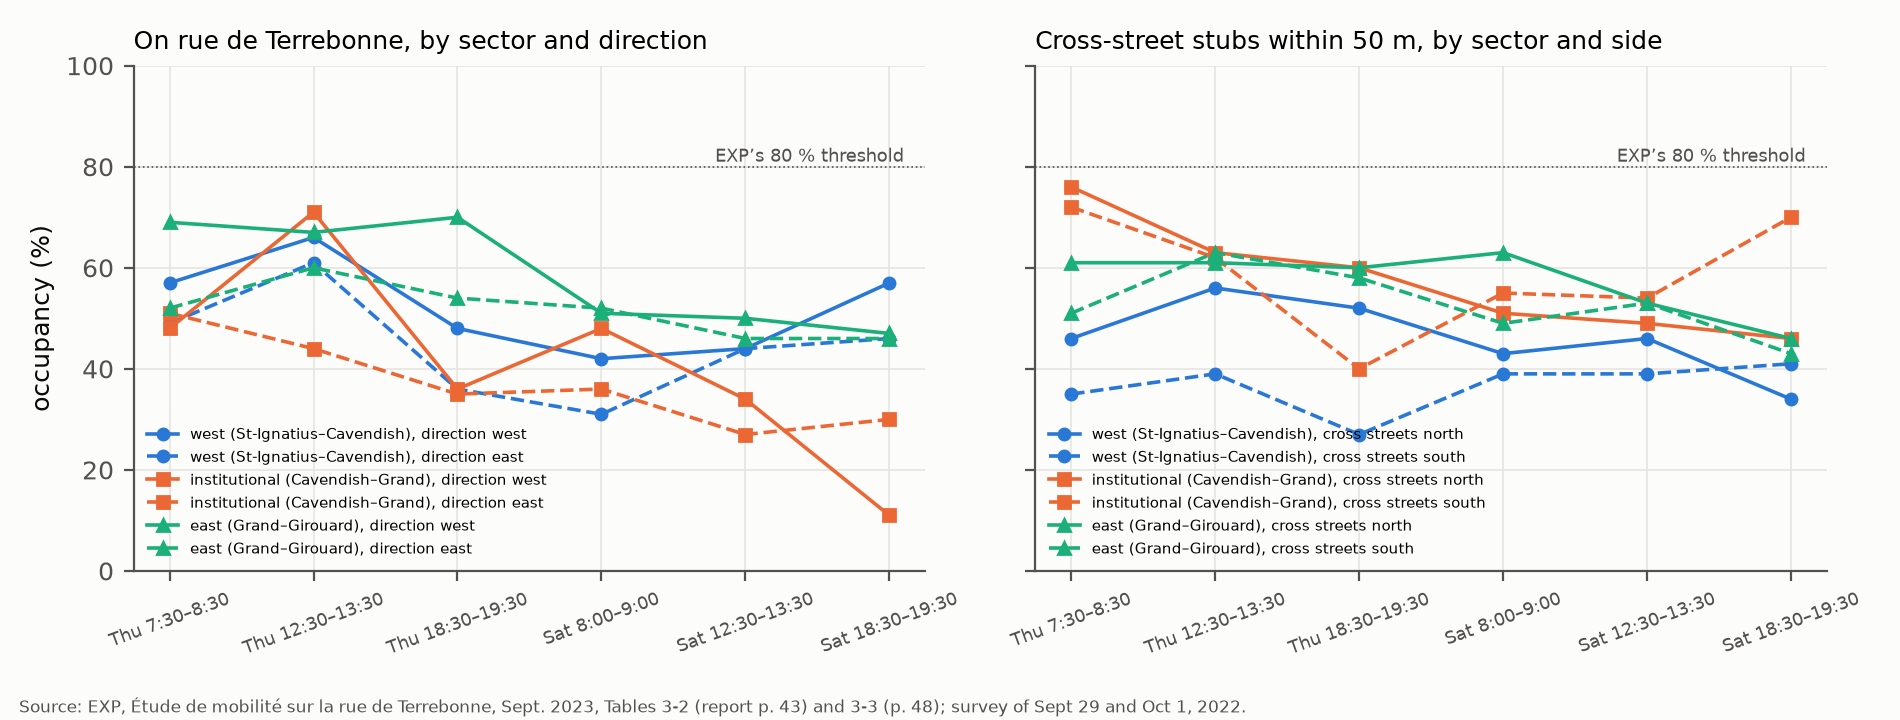
\includegraphics[width=1.0\textwidth]{figures/exp_occupancy_en.png}\caption{Occupancy by sector, direction or side, and period (EXP Tables 3-2 and 3-3). Dotted line: the 80\,\% threshold EXP uses.}\label{fig:exp_occupancy}\end{figure}
\begin{figure}[htbp]\centering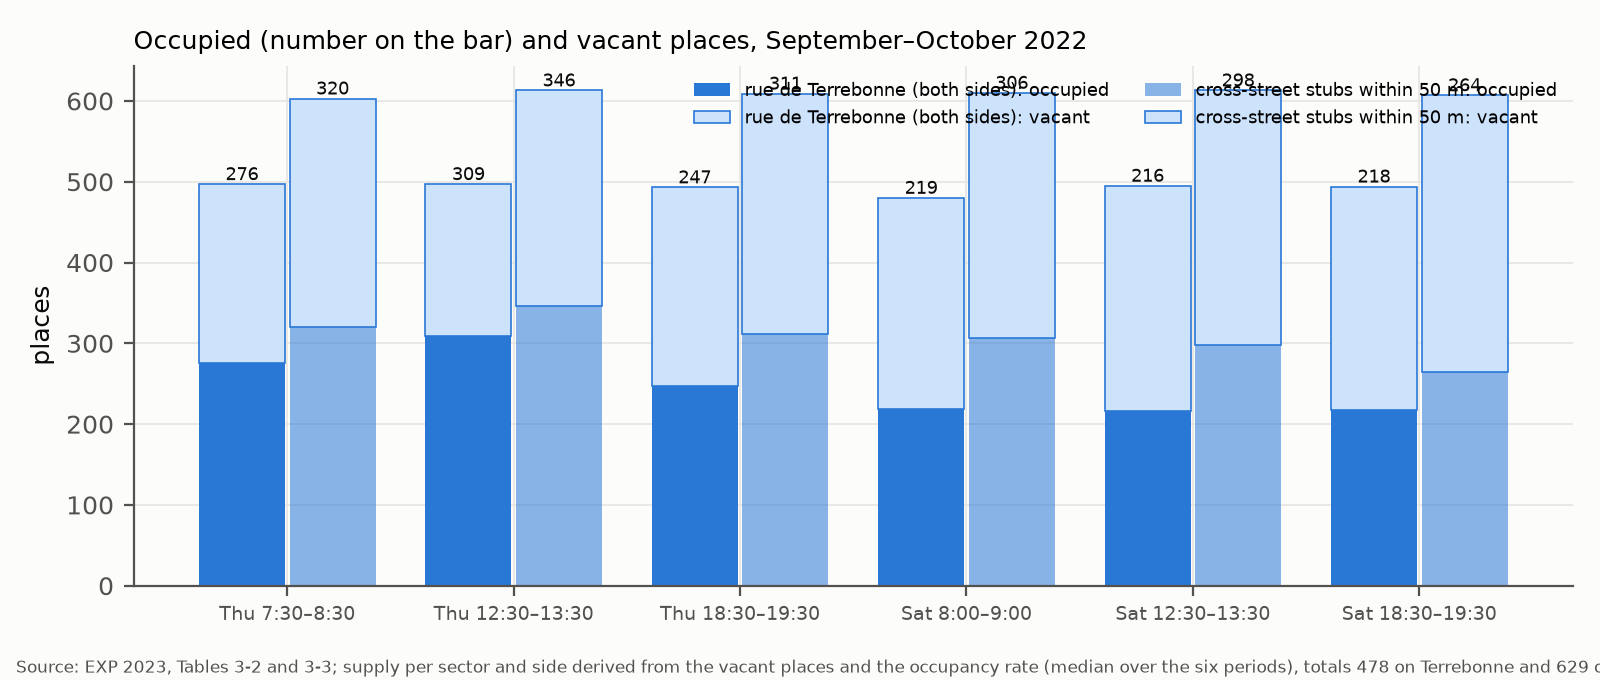
\includegraphics[width=0.9\textwidth]{figures/exp_occupied_vacant_en.png}\caption{Occupied (number on the bar) and vacant places per period on Terrebonne and on the cross-street stubs.}\label{fig:exp_occupied_vacant}\end{figure}

\subsection{The cars at the curbs, 2015 and the orthophoto}
\begin{table}[htbp]\centering\small\caption{Cars at Terrebonne\textquoteright{}s curbs by sector, both sides, against EXP\textquoteright{}s supply and its Thursday-evening count.}\label{tab:sec}
\resizebox{\textwidth}{!}{\begin{tabular}{@{}lrrrrrr@{}}\toprule sector & blocks & EXP supply (derived) & EXP occupied, Thu 18:30 & LiDAR night 2015 & night / supply & orthophoto, day\\ \midrule
residential west & 12 & 189 & 79 & 52 & 28\,\% & 62 \\
institutional & 5 & 83 & 30 & 29 & 35\,\% & 23 \\
residential east & 12 & 223 & 138 & 102 & 46\,\% & 73 \\
\bottomrule\end{tabular}}\end{table}
The 2015 weeknight (a leaf-on night of unknown week, both curbs available, before the lane) holds 183 cars on the 2,410~m of the lane, 37\,\% of the 2022 supply, against a nominal capacity of about 803 at 6~m per car. The gradient runs east: 28\,\% of supply in the west sector, 35\,\% in the institutional sector, 46\,\% in the east, as in EXP\textquoteright{}s evening rates. The busiest blocks that night were Montclair--Walkley (16), de Hampton--Royal (15), Grand--Beaconsfield (12), Hingston--de Hampton (12). The daytime orthophoto holds 158, almost all on the south curb, which says more about the hour and the shadows than about demand. On the side the winter layout converts to parking (north west of Cavendish, south east of it) the night count is 98 and the day count 90.
\begin{figure}[htbp]\centering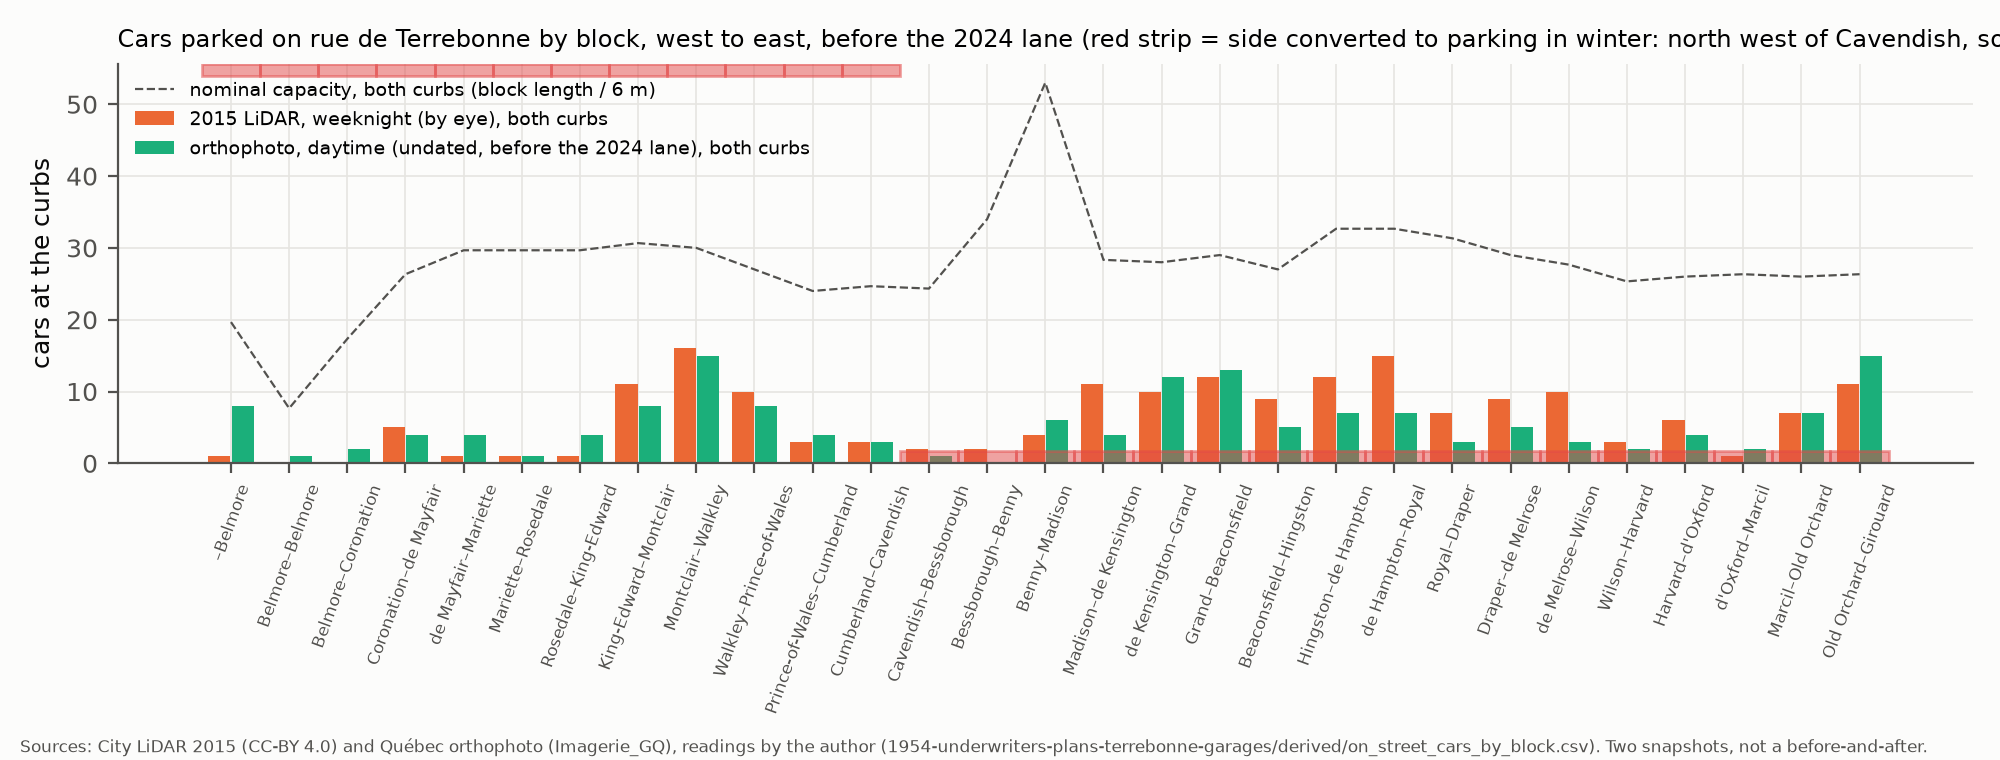
\includegraphics[width=1.0\textwidth]{figures/curb_cars_by_block_en.png}\caption{Cars at the curbs by block, west to east: the 2015 LiDAR night (by eye) and the daytime orthophoto, both curbs; dashed: nominal capacity at 6 m per car; red strip: the side converted to parking in winter.}\label{fig:curb_cars_by_block}\end{figure}

\textbf{Against the supply that remains.} The 2024 layout kept one parking band, of the order of 239 places (EXP counted 230 and 248 per direction). The two measurements of demand before the lane, 183 cars on a 2015 night and 247 on a 2022 Thursday evening, bracket that figure. In aggregate, the demand measured before the lane is of the order of the supply that remains on one side; by sector it is below it in the west and institutional sectors and near it in the east, before counting the 298 places EXP found vacant on the stubs at the same evening hour. Whether the street is fuller today than those measurements suggest cannot be known from them: no occupancy count has been made since the lane was built.

\subsection{Off-street parking: a ground truth for one survey question}
\begin{figure}[htbp]\centering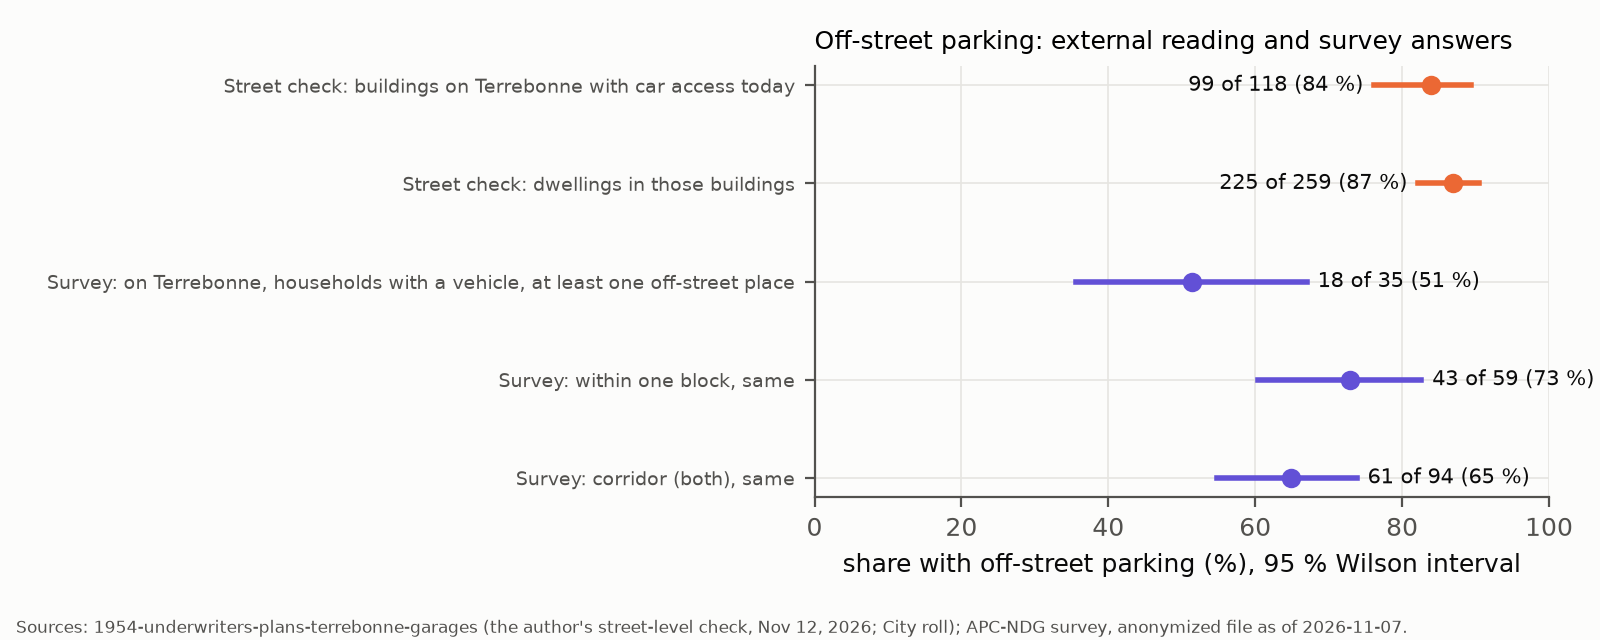
\includegraphics[width=0.9\textwidth]{figures/offstreet_share_en.png}\label{fig:offstreet_share}\end{figure}
The plans-and-imagery reading finds a garage or driveway at 89 of 123 buildings (72\,\%, interval 64--80\,\%) and for 188 of 268 dwellings (70\,\%); north side 70 of 89, south side 19 of 34. Survey respondents on Terrebonne with a vehicle report at least one off-street place in 18 of 35 cases (51\,\%, 36--67\,\%), those within a block in 43 of 59 (73\,\%). The on-street figure sits at the low edge of its interval against the reading. Two readings fit: households without off-street parking on Terrebonne were more likely to answer, which is what a survey about parking would be expected to do; or some respondents with a driveway did not count it (the question asked for places « built for a vehicle now »). Within a block, the survey and the reading agree, though the reading does not cover the cross streets. Either way, the survey\textquoteright{}s parking answers should not be read as shares of the street\textquoteright{}s households.

\subsection{The survey\textquoteright{}s demand floor}
\begin{table}[htbp]\centering\small\caption{The survey\textquoteright{}s parking answers by group (anonymized file as of 2026-11-07). Street parkers ticked a street for last night; hardship strict / loose as in the filing.}\label{tab:sv}
\resizebox{\textwidth}{!}{\begin{tabular}{@{}lrrrrrrrr@{}}\toprule group & respondents & with a vehicle & off-street place (of answered) & parked own off-street & on Terrebonne & cross street within a block & street parkers & hardship strict / loose\\ \midrule
on Terrebonne & 37 & 35 & 18 of 35 & 15 & 9 & 9 & 22 & 17 / 19 \\
within one block & 72 & 59 & 43 of 59 & 25 & 6 & 32 & 38 & 18 / 28 \\
corridor (both) & 109 & 94 & 61 of 94 & 40 & 15 & 41 & 60 & 35 / 47 \\
all respondents & 206 & 157 & 106 of 156 & 75 & 16 & 56 & 82 & 43 / 64 \\
\bottomrule\end{tabular}}\end{table}
\begin{figure}[htbp]\centering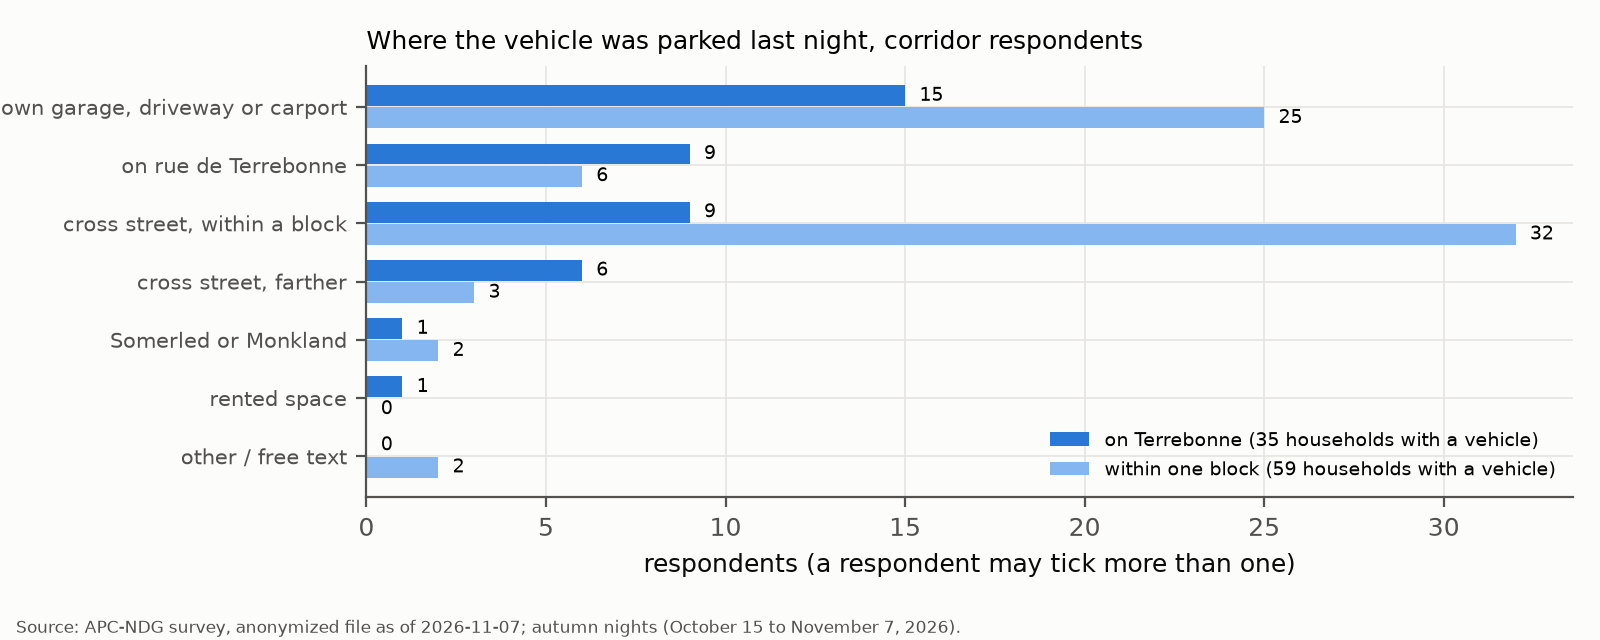
\includegraphics[width=0.9\textwidth]{figures/survey_parked_last_night_en.png}\label{fig:survey_parked_last_night}\end{figure}
Of the 109 corridor respondents, 94 keep a vehicle; 60 parked on a street the night before (15 on Terrebonne, 41 on a cross street within a block), and of those 35 met the strict hardship criterion and 47 the loose one. On Terrebonne itself, 22 of 37 respondents are street parkers and 17 of them report strict hardship; 17 of the 22 have no off-street place of their own. These are floors under the population, in the sense of the filing: at least this many answered this way.

\subsection{The population}
The roll holds 573 dwellings in 185 units with a Terrebonne address along the lane, and 5,029 dwellings in 2,316 units within the Somerled--Monkland band (bounding-box extract, clipped near Girouard on the north side). The survey reached 6\,\% of the dwellings on the street and 1\,\% of those within a block. The plans-and-imagery reading covers 268 of the 573 dwellings on the street (houses and plexes on the sheets available; the apartment blocks and the missing sheet are outside it).

\subsection{The winters}
\begin{table}[htbp]\centering\small\caption{Nights with a snow-removal constraint on parking, December 1 to March 31, five winters (borough; sector CDN-301).}\label{tab:win}
\begin{tabular}{@{}lrrrrr@{}}\toprule winter & loading, borough & loading, sector & storm-to-loading, borough & storm-to-loading, sector & snow days $\geq 2.5$ cm\\ \midrule
2021–22 & 27 & 26 & 36 & 36 & 46 \\
2022–23 & 27 & 25 & 34 & 33 & 48 \\
2023–24 & 12 & 10 & 18 & 17 & 31 \\
2024–25 & 27 & 25 & 32 & 32 & 57 \\
2025–26 & 24 & 30 & 36 & 44 & 54 \\
\bottomrule\end{tabular}\end{table}
\begin{figure}[htbp]\centering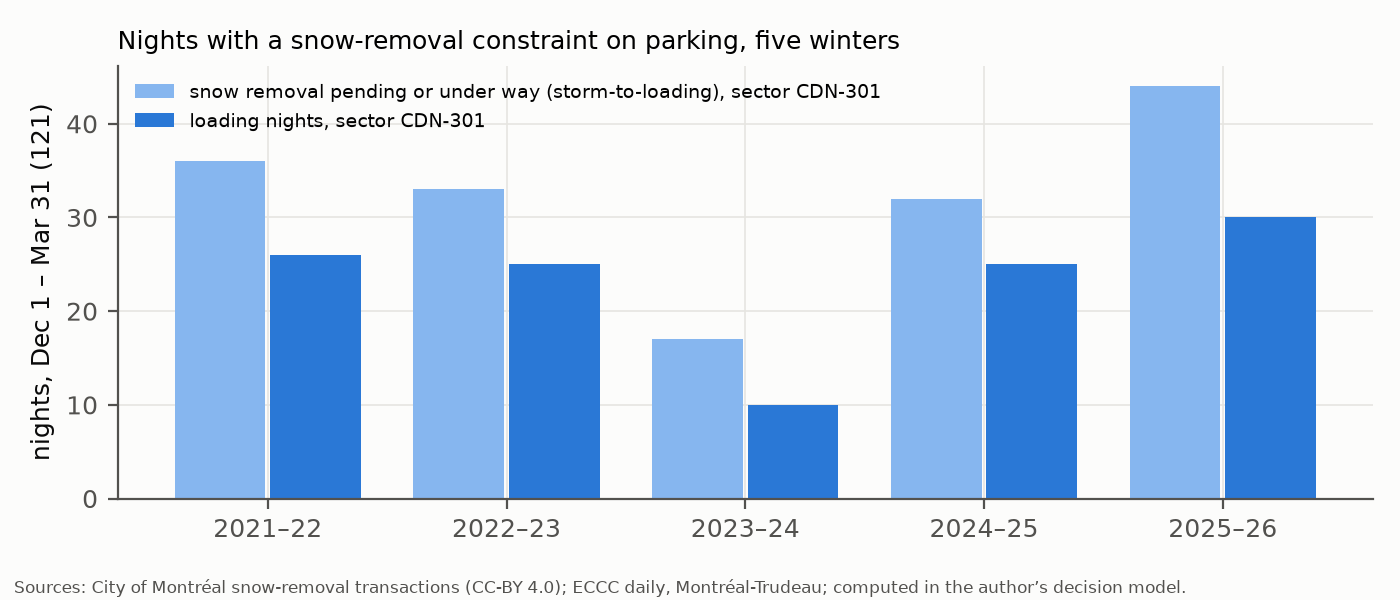
\includegraphics[width=0.8\textwidth]{figures/winter_constraint_nights_en.png}\label{fig:winter_constraint_nights}\end{figure}
The hardship questions ask about a typical winter evening and about the days after a storm or during loading. Over five winters the second condition held on about 32 of 121 nights in the sector, 23 of them with loading itself, with stretches of three weeks or more without it every winter. The survey cannot say how often a given respondent met the condition; the record says how often the condition existed.

\section{Discussion}
\textbf{What the external data settle.} Before the lane, parking on Terrebonne was measured twice and found about one-third to one-half full at the hours measured, with the east sector fuller than the west and ample room on the cross-street stubs. Seven in ten dwellings on the street have off-street parking. The supply that remains on one side today is of the order of the demand measured then. Those are measurements, and the survey\textquoteright{}s counts sit inside them: 60 street parkers among 5,602 dwellings is a floor, not a rate, and the off-street check shows the sample tilted, on the street itself, toward households that park on the street.

\textbf{What they do not.} The present occupancy, with the lane in place, is unmeasured: the borough has counted nothing since 2022, the survey\textquoteright{}s « last night » is an autumn night reported by respondents, and the 2015 night is a single snapshot with both curbs open. The hardship counts have no external check at all, only a record of how often the triggering conditions occur. The first parking analysis commissioned since 2022 (EXP\textquoteright{}s mandate of October 6, 2026, due November 27) is an analysis of supply, « cases existantes, ajoutées ou retranchées », not of occupancy.

\textbf{What would close the gap.} A night occupancy count on Terrebonne\textquoteright{}s remaining band and on the cross streets within a block, repeated on a few weeknights including one with snow removal pending, would give the measurement the 2022 survey gave for the pre-lane street; extending the garage-and-driveway reading to the first block of each cross street would give the within-a-block respondents the same ground truth the on-street respondents have.

\section{Reproducibility}
\texttt{parking\_analysis.py} reads the sources in place and writes \texttt{summary.json} (every number quoted here), \texttt{exp2022\_occupancy\_by\_period.csv}, \texttt{survey\_parking\_by\_group.csv} and the figures; \texttt{exp2023\_parking\_tables\_transcribed.csv} is the hand transcription of EXP\textquoteright{}s Tables 3-2 and 3-3 with their pages; \texttt{build\_docs.py} writes this note, the deck and the lay summaries. Generated 2026-11-07 11:24.
\end{document}
